%%%%%%%%%%%%%%%%%%%%%%%%%%%%
%%  Componenti del front end
%%%%%%%%%%%%%%%%%%%%%%%%%%%%



\subsection{\nogloxy{swedesigner::client}}
\label{\nogloxy{swedesigner::client}}
\subsubsection{Informazioni generali}
\begin{figure}[H]
	\makebox[\textwidth][c]{
	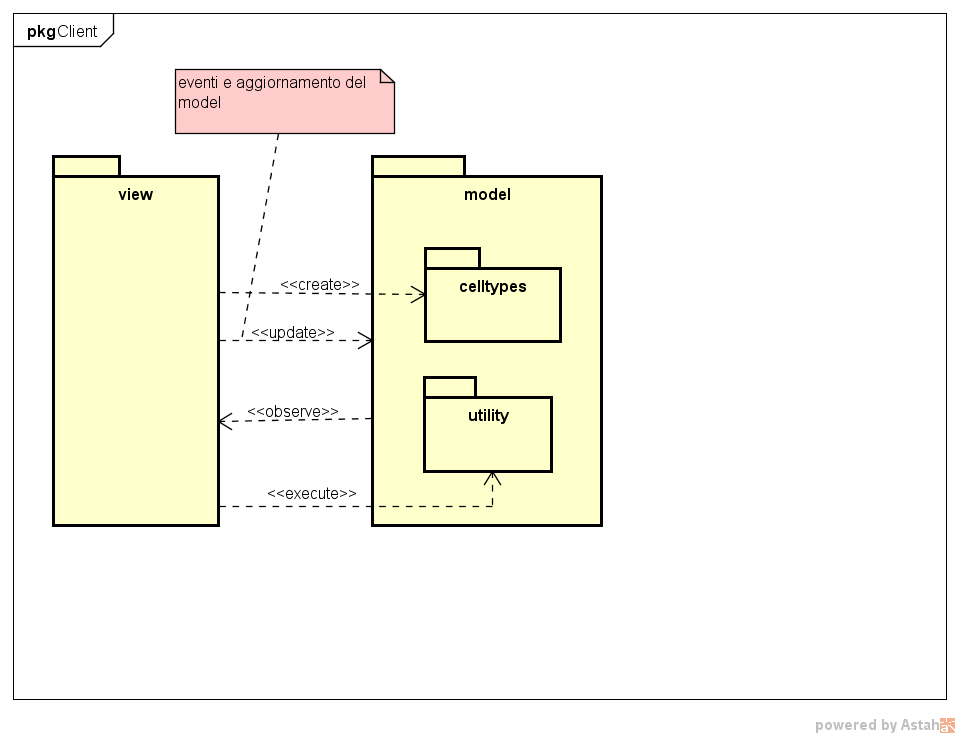
\includegraphics[width=1\textwidth]{img/client_pkg}}
	\caption{Diagramma package client}
\end{figure}
\begin{itemize}
\item \textbf{Descrizione}\\
Questo package descrive le componenti del \emph{front end}, scritte in JavaScript.
\item \textbf{Padre}: \hyperref[\nogloxy{swedesigner}]{\nogloxy{\texttt{swedesigner}}}
\item \textbf{Package contenuti}:
\begin{itemize}
\item \hyperref[\nogloxy{swedesigner::client::collection}]{\nogloxy{\texttt{collection}}}\\
Questo package descrive le classi che contengono delle collection (secondo la visione di \backbonejs). Ulteriori considerazioni sulla visione del pattern MVC sono contenute nell'appendice \ref{sec:app_creaz}.
\item \hyperref[\nogloxy{swedesigner::client::model}]{\nogloxy{\texttt{model}}}\\
Questo package contiene i modelli di dati usati dal client per rappresentare l'informazione manipolata dall'utente.
\item \hyperref[\nogloxy{swedesigner::client::view}]{\nogloxy{\texttt{view}}}\\
Questo package raccoglie le classi che rappresentano i menù laterali e il \texttt{canvas} visualizzati dal browser, che popolano template e si sottoscrivono alla view tramite un pattern Observer. (I template non sono contenuti in questo package.)
\end{itemize}
\end{itemize}

\subsection{\nogloxy{swedesigner::client::collection}}
\label{\nogloxy{swedesigner::client::collection}}
\subsubsection{Informazioni generali}
\begin{itemize}
\item \textbf{Descrizione}\\
Questo package descrive le classi che contengono delle collection (secondo la visione di \backbonejs). Ulteriori considerazioni sulla visione del pattern MVC sono contenute nell'appendice \ref{sec:app_creaz}.
\item \textbf{Padre}: \hyperref[\nogloxy{swedesigner::client}]{\nogloxy{\texttt{client}}}
\end{itemize}

\subsection{\nogloxy{swedesigner::client::model}}
\label{\nogloxy{swedesigner::client::model}}
\subsubsection{Informazioni generali}
\begin{figure}[H]
	\makebox[\textwidth][c]{
	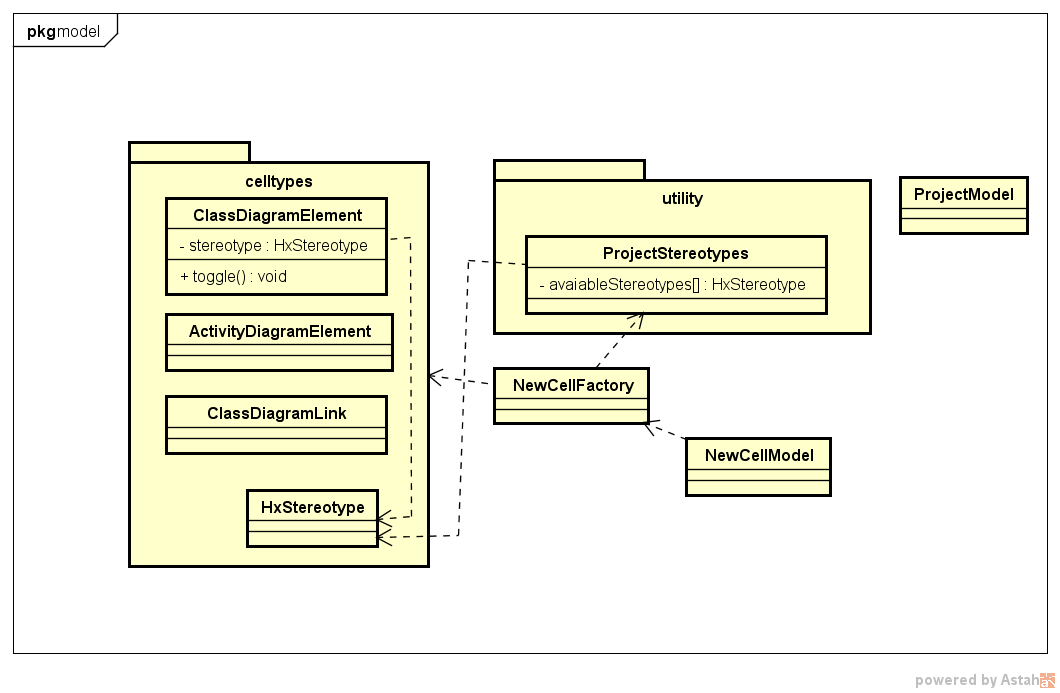
\includegraphics[width=1\textwidth]{img/client_model}}
	\caption{Diagramma package client::model}
\end{figure}
\begin{itemize}
\item \textbf{Descrizione}\\
Questo package contiene i modelli di dati usati dal client per rappresentare l'informazione manipolata dall'utente.
\item \textbf{Padre}: \hyperref[\nogloxy{swedesigner::client}]{\nogloxy{\texttt{client}}}
\item \textbf{Package contenuti}:
\begin{itemize}
\item \hyperref[\nogloxy{swedesigner::client::model::celltypes}]{\nogloxy{\texttt{celltypes}}}\\
Questo package contiene la definizione del modello degli elementi grafici dell'applicazione (e.g. diagrammi delle classi, blocchi condizionali\dots). 
\item \hyperref[\nogloxy{swedesigner::client::model::utility}]{\nogloxy{\texttt{utility}}}\\
Questo package racchiude le classi che definiscono i principali comandi dell'applicazione; esse fanno parte di un unico pattern Command, usato dalla \texttt{AppView} principale.
\end{itemize}
\end{itemize}
\subsubsection{Classi}
\subsubsubsection{\nogloxy{swedesigner::client::model::NewCellFactory}}
\label{\nogloxy{swedesigner::client::model::NewCellFactory}}
\begin{itemize}
\item \textbf{Descrizione}\\
questa classe si occupa di fornire un'istanza di una cella del tipo richiesto da \texttt{NewCellModel}. 
\item \textbf{Utilizzo}\\
viene utilizzata da \texttt{NewCellModel} che richiede una nuova cella (blocco o relazione) per avere un'istanza del blocco richiesto. Il design pattern descritto da questa classe è un Factory Pattern, come spiegato nel libro \emph{Learning Javascript Design Patterns} (\url{addyosmani.com/resources/essentialjsdesignpatterns/book/}).
\item \textbf{Relazioni con altre classi}:
\begin{itemize}
\item \textit{IN} \hyperref[\nogloxy{swedesigner::client::model::celltypes::activity::ActivityDiagramElement}]{\nogloxy{\texttt{ActivityDiagramElement}}}\\
questa classe è la base di tutte le classi che rappresentano i blocchi del diagramma delle attività.
\item \textit{IN} \hyperref[\nogloxy{swedesigner::client::model::NewCellModel}]{\nogloxy{\texttt{NewCellModel}}}\\
questa classe si occupa di fornire tutti i tipi di cell (tutti i blocchi e relazioni) da poter inserire nel diagramma corrente (o classi o attività).
\item \textit{OUT} \hyperref[\nogloxy{swedesigner::client::model::celltypes::class::ClassDiagramElement}]{\nogloxy{\texttt{ClassDiagramElement}}}\\
questa classe è la base di tutte le classi che rappresentano gli elementi del diagramma delle classi.
\end{itemize}
\end{itemize}

\subsubsubsection{\nogloxy{swedesigner::client::model::NewCellModel}}
\label{\nogloxy{swedesigner::client::model::NewCellModel}}
\begin{itemize}
\item \textbf{Descrizione}\\
questa classe si occupa di fornire tutti i tipi di cell (tutti i blocchi e relazioni) da poter inserire nel diagramma corrente (o classi o attività).
\item \textbf{Utilizzo}\\
utilizza \texttt{NewCellFactory} per recuperare una cell del tipo richiesto da \texttt{NewCellView}. Quest'ultima utilizza \texttt{NewCellModel} come modello da dove recuperare tutti i blocchi/relazioni che l'utente può inserire nel diagramma corrente.
\item \textbf{Relazioni con altre classi}:
\begin{itemize}
\item \textit{IN} \hyperref[\nogloxy{swedesigner::client::view::NewCellView}]{\nogloxy{\texttt{NewCellView}}}\\
questa classe si occupa di visualizzare tutti i possibili blocchi e relazioni che si possono inserire nel diagramma delle classi o delle attività.
\item \textit{OUT} \hyperref[\nogloxy{swedesigner::client::model::NewCellFactory}]{\nogloxy{\texttt{NewCellFactory}}}\\
questa classe si occupa di fornire un'istanza di una cella del tipo richiesto da \texttt{NewCellModel}. 
\end{itemize}
\end{itemize}

\subsubsubsection{\nogloxy{swedesigner::client::model::ProjectCommand}}
\label{\nogloxy{swedesigner::client::model::ProjectCommand}}
\begin{itemize}
\item \textbf{Descrizione}\\
questa interfaccia descrive la struttura di un comando che viene chiamato da \texttt{AppView} quando l'utente decide di creare un nuovo progetto, di caricarne uno esistente, di salvarlo o di generare il codice dal diagramma. Il pattern realizzato è il pattern Command.
\item \textbf{Utilizzo}\\
viene utilizzata da \texttt{AppView}, la quale poi chiederà comandi concreti in base all'input richiesto dall'utente.
\item \textbf{Relazioni con altre classi}:
\begin{itemize}
\item \textit{IN} \hyperref[\nogloxy{swedesigner::client::view::AppView}]{\nogloxy{\texttt{AppView}}}\\
questa classe si occupa di gestire l'intera view dell'applicazione, componendo l'interfaccia principale e richiamando le altre view tramite il sistema a template di \backbonejs{}.
\item \textit{OUT} \hyperref[\nogloxy{swedesigner::client::model::ProjectModel}]{\nogloxy{\texttt{ProjectModel}}}\\
questa classe ci permette di aggiungere della logica alla collezione di tutti i diagrammi che possediamo.
\end{itemize}
\end{itemize}

\subsubsubsection{\nogloxy{swedesigner::client::model::ProjectModel}}
\label{\nogloxy{swedesigner::client::model::ProjectModel}}
\begin{itemize}
\item \textbf{Descrizione}\\
questa classe ci permette di aggiungere della logica alla collezione di tutti i diagrammi che possediamo.
\item \textbf{Utilizzo}\\
essa è istanziata da \texttt{ProjectView} e possiede \texttt{DiagramCollection}. È possibile interagire con questo modello anche tramite \texttt{ProjectCommand}, per permettere l'implementazione di funzionalità globali dell'applicazione (e.g. salvataggio e caricamento).
\item \textbf{Relazioni con altre classi}:
\begin{itemize}
\item \textit{IN} \hyperref[\nogloxy{swedesigner::client::model::ProjectCommand}]{\nogloxy{\texttt{ProjectCommand}}}\\
questa interfaccia descrive la struttura di un comando che viene chiamato da \texttt{AppView} quando l'utente decide di creare un nuovo progetto, di caricarne uno esistente, di salvarlo o di generare il codice dal diagramma. Il pattern realizzato è il pattern Command.
\item \textit{IN} \hyperref[\nogloxy{swedesigner::client::view::AppView}]{\nogloxy{\texttt{AppView}}}\\
questa classe si occupa di gestire l'intera view dell'applicazione, componendo l'interfaccia principale e richiamando le altre view tramite il sistema a template di \backbonejs{}.
\item \textit{IN} \hyperref[\nogloxy{swedesigner::client::view::ProjectView}]{\nogloxy{\texttt{ProjectView}}}\\
questa classe rappresenta l'area di disegno principale dell'applicazione, che necessita di essere cambiata tra diagramma delle classi e diagramma delle attività. 
\end{itemize}
\end{itemize}
\subsection{\nogloxy{swedesigner::client::model::celltypes}}
\label{\nogloxy{swedesigner::client::model::celltypes}}
\subsubsection{Informazioni generali}
\begin{figure}[H]
	\makebox[\textwidth][c]{
	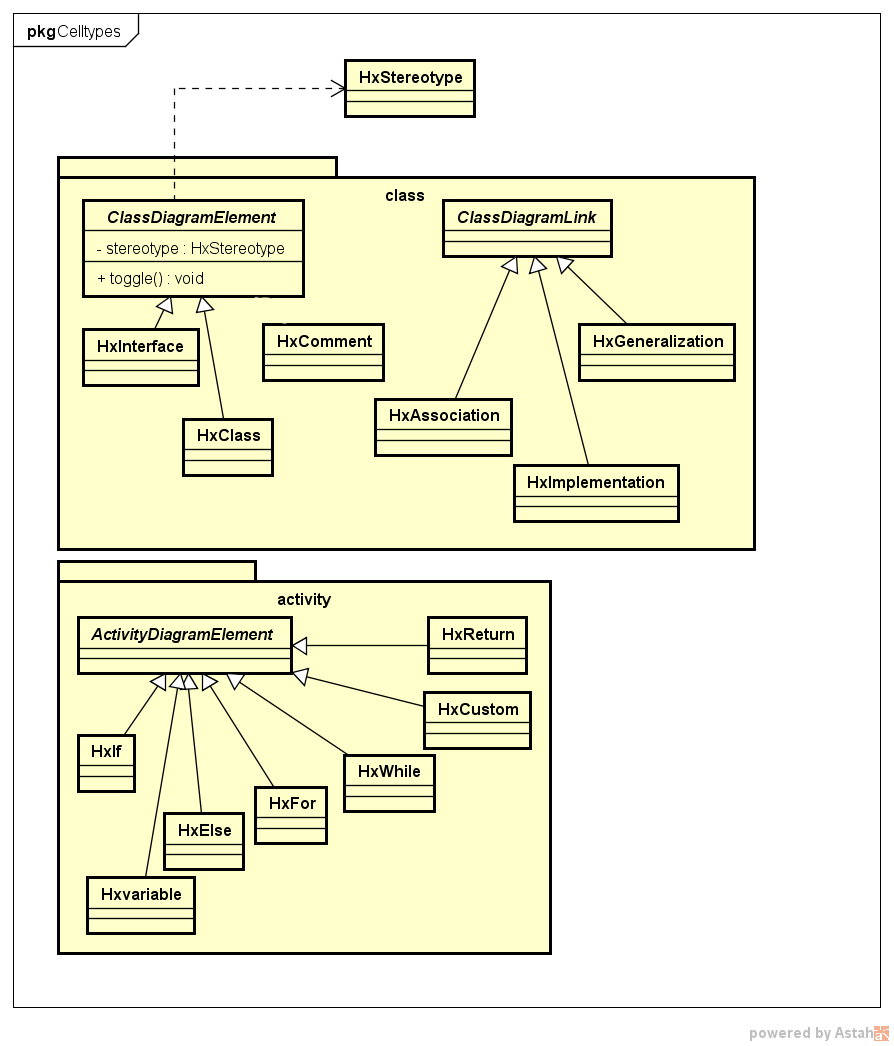
\includegraphics[width=1\textwidth]{img/client_cellTypes}}
	\caption{Diagramma package client::model::celltypes}
\end{figure}
\begin{itemize}
\item \textbf{Descrizione}\\
Questo package contiene la definizione del modello degli elementi grafici dell'applicazione (e.g. diagrammi delle classi, blocchi condizionali\dots). 
\item \textbf{Padre}: \hyperref[\nogloxy{swedesigner::client::model}]{\nogloxy{\texttt{model}}}
\item \textbf{Package contenuti}:
\begin{itemize}
\item \hyperref[\nogloxy{swedesigner::client::model::celltypes::activity}]{\nogloxy{\texttt{activity}}}\\
Questo package contiene la definizione del modello degli elementi specifi del diagramma delle classi dell'applicazione.
\item \hyperref[\nogloxy{swedesigner::client::model::celltypes::class}]{\nogloxy{\texttt{class}}}\\
Questo package contiene la definizione del modello degli elementi specifi del diagramma delle classi dell'applicazione.
\end{itemize}
\end{itemize}
\subsubsection{Classi}
\subsubsubsection{\nogloxy{swedesigner::client::model::celltypes::HxStereotype}}
\label{\nogloxy{swedesigner::client::model::celltypes::HxStereotype}}
\begin{itemize}
\item \textbf{Descrizione}\\
questa classe rappresenta le caratteristiche dello stereotipo che viene assegnato ad un \texttt{ClassDiagramElement} come i meta-attributi e meta-metodi, i quali sono essere ridefiniti dalla classe o interfaccia implementata tramite \proj{}. 
\item \textbf{Utilizzo}\\
ogni elemento possiederà un unico stereotipo per semplificare l'implementazione di \proj{}. Gli stereotipi disponibili sono presenti all'interno della classe \texttt{ProjectStereotypes} (all'interno di \emph{model::utility}).
\item \textbf{Relazioni con altre classi}:
\begin{itemize}
\item \textit{IN} \hyperref[\nogloxy{swedesigner::client::model::celltypes::class::ClassDiagramElement}]{\nogloxy{\texttt{ClassDiagramElement}}}\\
questa classe è la base di tutte le classi che rappresentano gli elementi del diagramma delle classi.
\item \textit{IN} \hyperref[\nogloxy{swedesigner::client::model::utility::ProjectStereotypes}]{\nogloxy{\texttt{ProjectStereotypes}}}\\
questa classe contiene al suo interno i possibili stereotipi utilizzabili recuperati dal server in modo asincrono. Conterrà una lista di elementi \textt{HxStereotype}.
\end{itemize}
\end{itemize}
\subsection{\nogloxy{swedesigner::client::model::celltypes::activity}}
\label{\nogloxy{swedesigner::client::model::celltypes::activity}}
\subsubsection{Informazioni generali}
\begin{itemize}
\item \textbf{Descrizione}\\
Questo package contiene la definizione del modello degli elementi specifi del diagramma delle classi dell'applicazione.
\item \textbf{Padre}: \hyperref[\nogloxy{swedesigner::client::model::celltypes}]{\nogloxy{\texttt{celltypes}}}
\end{itemize}
\subsubsection{Classi}
\subsubsubsection{\nogloxy{swedesigner::client::model::celltypes::activity::ActivityDiagramElement}}
\label{\nogloxy{swedesigner::client::model::celltypes::activity::ActivityDiagramElement}}
\begin{itemize}
\item \textbf{Descrizione}\\
questa classe è la base di tutte le classi che rappresentano i blocchi del diagramma delle attività.
\item \textbf{Utilizzo}\\
estende sottotipi della classe \texttt{Element} (la quale deriva a sua volta da \texttt{Cell})  di \jointjs{} e viene estesa da tutte le classi specifiche di ogni blocco del diagramma delle attività. Questa classe è indirettamente correlata a \texttt{NewCellFactory}.
\item \textbf{Sottoclassi}:
\begin{itemize}
\item \hyperref[\nogloxy{swedesigner::client::model::celltypes::activity::HxCustom}]{\nogloxy{\texttt{HxCustom}}}
\item \hyperref[\nogloxy{swedesigner::client::model::celltypes::activity::HxElse}]{\nogloxy{\texttt{HxElse}}}
\item \hyperref[\nogloxy{swedesigner::client::model::celltypes::activity::HxFor}]{\nogloxy{\texttt{HxFor}}}
\item \hyperref[\nogloxy{swedesigner::client::model::celltypes::activity::HxIf}]{\nogloxy{\texttt{HxIf}}}
\item \hyperref[\nogloxy{swedesigner::client::model::celltypes::activity::HxReturn}]{\nogloxy{\texttt{HxReturn}}}
\item \hyperref[\nogloxy{swedesigner::client::model::celltypes::activity::HxVariable}]{\nogloxy{\texttt{HxVariable}}}
\item \hyperref[\nogloxy{swedesigner::client::model::celltypes::activity::HxWhile}]{\nogloxy{\texttt{HxWhile}}}
\end{itemize}
\item \textbf{Relazioni con altre classi}:
\begin{itemize}
\item \textit{OUT} \hyperref[\nogloxy{swedesigner::client::model::NewCellFactory}]{\nogloxy{\texttt{NewCellFactory}}}\\
questa classe si occupa di fornire un'istanza di una cella del tipo richiesto da \texttt{NewCellModel}. 
\end{itemize}
\end{itemize}

\subsubsubsection{\nogloxy{swedesigner::client::model::celltypes::activity::HxCustom}}
\label{\nogloxy{swedesigner::client::model::celltypes::activity::HxCustom}}
\begin{itemize}
\item \textbf{Descrizione}\\
questa classe rappresenta il blocco custom del diagramma delle attività che permette all'utente di inserire liberamente codice nel linguaggio target scelto.
\item \textbf{Utilizzo}\\
la classe \texttt{NewCellFactory} ritorna un'istanza di questa classe ogni volta che l'utente richiede un nuovo blocco di codice personalizzato.
\item \textbf{Classi ereditate}:
\begin{itemize}
\item \hyperref[\nogloxy{swedesigner::client::model::celltypes::activity::ActivityDiagramElement}]{\nogloxy{\texttt{ActivityDiagramElement}}}
\end{itemize}
\end{itemize}

\subsubsubsection{\nogloxy{swedesigner::client::model::celltypes::activity::HxElse}}
\label{\nogloxy{swedesigner::client::model::celltypes::activity::HxElse}}
\begin{itemize}
\item \textbf{Descrizione}\\
Questa classe rappresenta il blocco else del diagramma delle attività
\item \textbf{Utilizzo}\\
la classe \texttt{NewCellFactory} ritorna un'istanza di questa classe ogni volta che l'utente richiede un nuovo blocco \texttt{for}.
\item \textbf{Classi ereditate}:
\begin{itemize}
\item \hyperref[\nogloxy{swedesigner::client::model::celltypes::activity::ActivityDiagramElement}]{\nogloxy{\texttt{ActivityDiagramElement}}}
\end{itemize}
\end{itemize}

\subsubsubsection{\nogloxy{swedesigner::client::model::celltypes::activity::HxFor}}
\label{\nogloxy{swedesigner::client::model::celltypes::activity::HxFor}}
\begin{itemize}
\item \textbf{Descrizione}\\
questa classe rappresenta il blocco \texttt{for} del diagramma delle attività.
\item \textbf{Utilizzo}\\
la classe \texttt{NewCellFactory} ritorna un'istanza di questa classe ogni volta che l'utente richiede un nuovo blocco \texttt{for}.
\item \textbf{Classi ereditate}:
\begin{itemize}
\item \hyperref[\nogloxy{swedesigner::client::model::celltypes::activity::ActivityDiagramElement}]{\nogloxy{\texttt{ActivityDiagramElement}}}
\end{itemize}
\end{itemize}

\subsubsubsection{\nogloxy{swedesigner::client::model::celltypes::activity::HxIf}}
\label{\nogloxy{swedesigner::client::model::celltypes::activity::HxIf}}
\begin{itemize}
\item \textbf{Descrizione}\\
questa classe rappresenta il blocco \texttt{if} del diagramma delle attività.
\item \textbf{Utilizzo}\\
la classe \texttt{NewCellFactory} ritorna un'istanza di questa classe ogni volta che l'utente richiede un nuovo blocco \texttt{if}.
\item \textbf{Classi ereditate}:
\begin{itemize}
\item \hyperref[\nogloxy{swedesigner::client::model::celltypes::activity::ActivityDiagramElement}]{\nogloxy{\texttt{ActivityDiagramElement}}}
\end{itemize}
\end{itemize}

\subsubsubsection{\nogloxy{swedesigner::client::model::celltypes::activity::HxReturn}}
\label{\nogloxy{swedesigner::client::model::celltypes::activity::HxReturn}}
\begin{itemize}
\item \textbf{Descrizione}\\
questa classe rappresenta il blocco \emph{return} del diagramma delle attività.
\item \textbf{Utilizzo}\\
la classe \texttt{NewCellFactory} ritorna un'istanza di questa classe ogni volta che l'utente richiede un nuovo blocco \emph{return}.
\item \textbf{Classi ereditate}:
\begin{itemize}
\item \hyperref[\nogloxy{swedesigner::client::model::celltypes::activity::ActivityDiagramElement}]{\nogloxy{\texttt{ActivityDiagramElement}}}
\end{itemize}
\end{itemize}

\subsubsubsection{\nogloxy{swedesigner::client::model::celltypes::activity::HxVariable}}
\label{\nogloxy{swedesigner::client::model::celltypes::activity::HxVariable}}
\begin{itemize}
\item \textbf{Descrizione}\\
questa classe rappresenta il blocco di assegnazione o inizializzazione di una variabile o di chiamata di un metodo del diagramma delle attività.
\item \textbf{Utilizzo}\\
la classe \texttt{NewCellFactory} ritorna un'istanza di questa classe ogni volta che l'utente richiede un nuovo blocco variabile.
\item \textbf{Classi ereditate}:
\begin{itemize}
\item \hyperref[\nogloxy{swedesigner::client::model::celltypes::activity::ActivityDiagramElement}]{\nogloxy{\texttt{ActivityDiagramElement}}}
\end{itemize}
\end{itemize}

\subsubsubsection{\nogloxy{swedesigner::client::model::celltypes::activity::HxWhile}}
\label{\nogloxy{swedesigner::client::model::celltypes::activity::HxWhile}}
\begin{itemize}
\item \textbf{Descrizione}\\
questa classe rappresenta il blocco \emph{while} del diagramma delle attività.
\item \textbf{Utilizzo}\\
la classe \texttt{NewCellFactory} ritorna un'istanza di questa classe ogni volta che l'utente richiede un nuovo blocco \emph{while}.
\item \textbf{Classi ereditate}:
\begin{itemize}
\item \hyperref[\nogloxy{swedesigner::client::model::celltypes::activity::ActivityDiagramElement}]{\nogloxy{\texttt{ActivityDiagramElement}}}
\end{itemize}
\end{itemize}
\subsection{\nogloxy{swedesigner::client::model::celltypes::class}}
\label{\nogloxy{swedesigner::client::model::celltypes::class}}
\subsubsection{Informazioni generali}
\begin{itemize}
\item \textbf{Descrizione}\\
Questo package contiene la definizione del modello degli elementi specifi del diagramma delle classi dell'applicazione.
\item \textbf{Padre}: \hyperref[\nogloxy{swedesigner::client::model::celltypes}]{\nogloxy{\texttt{celltypes}}}
\end{itemize}
\subsubsection{Classi}
\subsubsubsection{\nogloxy{swedesigner::client::model::celltypes::class::ClassDiagramElement}}
\label{\nogloxy{swedesigner::client::model::celltypes::class::ClassDiagramElement}}
\begin{itemize}
\item \textbf{Descrizione}\\
questa classe è la base di tutte le classi che rappresentano gli elementi del diagramma delle classi.
\item \textbf{Utilizzo}\\
eredita da sottotipi della classe \texttt{Element} di \jointjs{} (la quale deriva a sua volta da \texttt{Cell}) e viene estesa da tutte le classi specifiche di ogni blocco del diagramma delle classi. Questa classe è indirettamente correlata con \texttt{NewCellFactory}, derivando da \texttt{Cell}.
\item \textbf{Sottoclassi}:
\begin{itemize}
\item \hyperref[\nogloxy{swedesigner::client::model::celltypes::class::HxClass}]{\nogloxy{\texttt{HxClass}}}
\item \hyperref[\nogloxy{swedesigner::client::model::celltypes::class::HxInterface}]{\nogloxy{\texttt{HxInterface}}}
\end{itemize}
\item \textbf{Relazioni con altre classi}:
\begin{itemize}
\item \textit{IN} \hyperref[\nogloxy{swedesigner::client::model::NewCellFactory}]{\nogloxy{\texttt{NewCellFactory}}}\\
questa classe si occupa di fornire un'istanza di una cella del tipo richiesto da \texttt{NewCellModel}. 
\item \textit{OUT} \hyperref[\nogloxy{swedesigner::client::model::celltypes::HxStereotype}]{\nogloxy{\texttt{HxStereotype}}}\\
questa classe rappresenta le caratteristiche dello stereotipo che viene assegnato ad un \texttt{ClassDiagramElement} come i meta-attributi e meta-metodi, i quali sono essere ridefiniti dalla classe o interfaccia implementata tramite \proj{}. 
\end{itemize}
\end{itemize}

\subsubsubsection{\nogloxy{swedesigner::client::model::celltypes::class::ClassDiagramLink}}
\label{\nogloxy{swedesigner::client::model::celltypes::class::ClassDiagramLink}}
\begin{itemize}
\item \textbf{Descrizione}\\
questa classe è la base di tutte le classi che rappresentano le relazioni tra gli elementi del diagramma delle classi.
\item \textbf{Utilizzo}\\
eredita dalla classe \texttt{Link} di \jointjs{} e viene estesa da tutte le classi specifiche di ogni relazione del diagramma delle classi.
\item \textbf{Sottoclassi}:
\begin{itemize}
\item \hyperref[\nogloxy{swedesigner::client::model::celltypes::class::HxAssociation}]{\nogloxy{\texttt{HxAssociation}}}
\item \hyperref[\nogloxy{swedesigner::client::model::celltypes::class::HxGeneralization}]{\nogloxy{\texttt{HxGeneralization}}}
\item \hyperref[\nogloxy{swedesigner::client::model::celltypes::class::HxImplementation}]{\nogloxy{\texttt{HxImplementation}}}
\end{itemize}
\end{itemize}

\subsubsubsection{\nogloxy{swedesigner::client::model::celltypes::class::HxAssociation}}
\label{\nogloxy{swedesigner::client::model::celltypes::class::HxAssociation}}
\begin{itemize}
\item \textbf{Descrizione}\\
Questa classe rappresenta una relazione associazione tra due blocchi del diagramma delle classi
\item \textbf{Utilizzo}\\
eredita dalla classe \texttt{ClassDiagramLink}. È indirettamente collegata a \texttt{NewCellFactory} in quanto è anch'essa una derivata di \texttt{Cell}.
\item \textbf{Classi ereditate}:
\begin{itemize}
\item \hyperref[\nogloxy{swedesigner::client::model::celltypes::class::ClassDiagramLink}]{\nogloxy{\texttt{ClassDiagramLink}}}
\end{itemize}
\end{itemize}

\subsubsubsection{\nogloxy{swedesigner::client::model::celltypes::class::HxClass}}
\label{\nogloxy{swedesigner::client::model::celltypes::class::HxClass}}
\begin{itemize}
\item \textbf{Descrizione}\\
questa classe rappresenta il blocco \texttt{class} del diagramma delle classi UML.
\item \textbf{Utilizzo}\\
la classe \texttt{NewCellFactory} ritorna un'istanza di questa classe ogni volta che l'utente richiede un nuovo elemento \emph{class}.
\item \textbf{Classi ereditate}:
\begin{itemize}
\item \hyperref[\nogloxy{swedesigner::client::model::celltypes::class::ClassDiagramElement}]{\nogloxy{\texttt{ClassDiagramElement}}}
\end{itemize}
\end{itemize}

\subsubsubsection{\nogloxy{swedesigner::client::model::celltypes::class::HxComment}}
\label{\nogloxy{swedesigner::client::model::celltypes::class::HxComment}}
\begin{itemize}
\item \textbf{Descrizione}\\
questa classe rappresenta la cella di commento del diagramma delle classi UML. Eredita da un tipo base di jointjs.
\item \textbf{Utilizzo}\\
la classe \texttt{NewCellFactory} ritorna un'istanza di questa classe ogni volta che l'utente richiede un nuovo commento.
\end{itemize}

\subsubsubsection{\nogloxy{swedesigner::client::model::celltypes::class::HxGeneralization}}
\label{\nogloxy{swedesigner::client::model::celltypes::class::HxGeneralization}}
\begin{itemize}
\item \textbf{Descrizione}\\
questa classe rappresenta la relazione di generalizzazione tra due celle del diagramma delle classi.
\item \textbf{Utilizzo}\\
eredita dalla classe \texttt{ClassDiagramLink}. È indirettamente collegata a \texttt{NewCellFactory} in quanto è anch'essa una derivata di \texttt{Cell}.
\item \textbf{Classi ereditate}:
\begin{itemize}
\item \hyperref[\nogloxy{swedesigner::client::model::celltypes::class::ClassDiagramLink}]{\nogloxy{\texttt{ClassDiagramLink}}}
\end{itemize}
\end{itemize}

\subsubsubsection{\nogloxy{swedesigner::client::model::celltypes::class::HxImplementation}}
\label{\nogloxy{swedesigner::client::model::celltypes::class::HxImplementation}}
\begin{itemize}
\item \textbf{Descrizione}\\
questa classe rappresenta la relazione di implementazione tra due celle del diagramma delle classi.
\item \textbf{Utilizzo}\\
eredita dalla classe \texttt{ClassDiagramLink}. È indirettamente collegata a \texttt{NewCellFactory} in quanto è anch'essa una derivata di \texttt{Cell}.
\item \textbf{Classi ereditate}:
\begin{itemize}
\item \hyperref[\nogloxy{swedesigner::client::model::celltypes::class::ClassDiagramLink}]{\nogloxy{\texttt{ClassDiagramLink}}}
\end{itemize}
\end{itemize}

\subsubsubsection{\nogloxy{swedesigner::client::model::celltypes::class::HxInterface}}
\label{\nogloxy{swedesigner::client::model::celltypes::class::HxInterface}}
\begin{itemize}
\item \textbf{Descrizione}\\
questa classe rappresenta il costrutto \emph{interface} del diagramma delle classi UML.
\item \textbf{Utilizzo}\\
la classe \texttt{NewCellFactory} ritorna un'istanza di questa classe ogni volta che l'utente richiede un nuovo elemento \emph{interface}.
\item \textbf{Classi ereditate}:
\begin{itemize}
\item \hyperref[\nogloxy{swedesigner::client::model::celltypes::class::ClassDiagramElement}]{\nogloxy{\texttt{ClassDiagramElement}}}
\end{itemize}
\end{itemize}
\subsection{\nogloxy{swedesigner::client::model::utility}}
\label{\nogloxy{swedesigner::client::model::utility}}
\subsubsection{Informazioni generali}
\begin{figure}[H]
	\makebox[\textwidth][c]{
	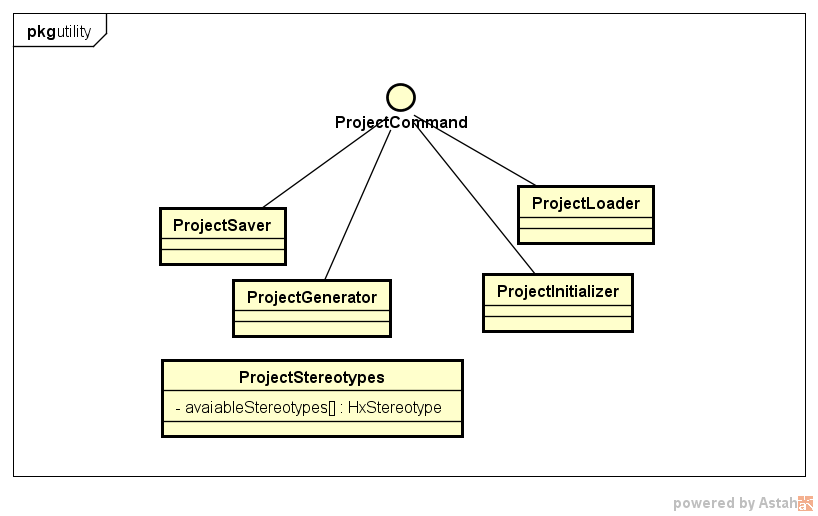
\includegraphics[width=1\textwidth]{img/client_utility}}
	\caption{Diagramma package client::model::utility}
\end{figure}
\begin{itemize}
\item \textbf{Descrizione}\\
Questo package racchiude le classi che definiscono i principali comandi dell'applicazione; esse fanno parte di un unico pattern Command, usato dalla \texttt{AppView} principale.
\item \textbf{Padre}: \hyperref[\nogloxy{swedesigner::client::model}]{\nogloxy{\texttt{model}}}
\end{itemize}
\subsubsection{Classi}
\subsubsubsection{\nogloxy{swedesigner::client::model::utility::ProjectStereotypes}}
\label{\nogloxy{swedesigner::client::model::utility::ProjectStereotypes}}
\begin{itemize}
\item \textbf{Descrizione}\\
questa classe contiene al suo interno i possibili stereotipi utilizzabili recuperati dal server in modo asincrono. Conterrà una lista di elementi \textt{HxStereotype}.
\item \textbf{Utilizzo}\\
\texttt{DetailsView} necessita degli stereotipi esistenti per permettere l'inserimento e la modifica dello stereotipo di una classe. È possibile che la \texttt{NewCellFactory} faccia una richiesta simile a questa classe, al fine di poter fornire all'utente la possibilità di inserire una classe già stereotipata. 
\item \textbf{Relazioni con altre classi}:
\begin{itemize}
\item \textit{IN} \hyperref[\nogloxy{swedesigner::client::view::DetailsView}]{\nogloxy{\texttt{DetailsView}}}\\
questa classe si occupa di visualizzare tutti i campi di un blocco o di una relazione (come il nome di una classe, i suoi attributi, la condizione di un blocco \texttt{if} o il blocco di partenza di una relazione) permettendone anche la modifica. È possibile anche specificare uno stereotipo per la classe.

\item \textit{OUT} \hyperref[\nogloxy{swedesigner::client::model::celltypes::HxStereotype}]{\nogloxy{\texttt{HxStereotype}}}\\
questa classe rappresenta le caratteristiche dello stereotipo che viene assegnato ad un \texttt{ClassDiagramElement} come i meta-attributi e meta-metodi, i quali sono essere ridefiniti dalla classe o interfaccia implementata tramite \proj{}. 
\end{itemize}
\end{itemize}
\subsection{\nogloxy{swedesigner::client::view}}
\label{\nogloxy{swedesigner::client::view}}
\subsubsection{Informazioni generali}
\begin{figure}[H]
	\makebox[\textwidth][c]{
	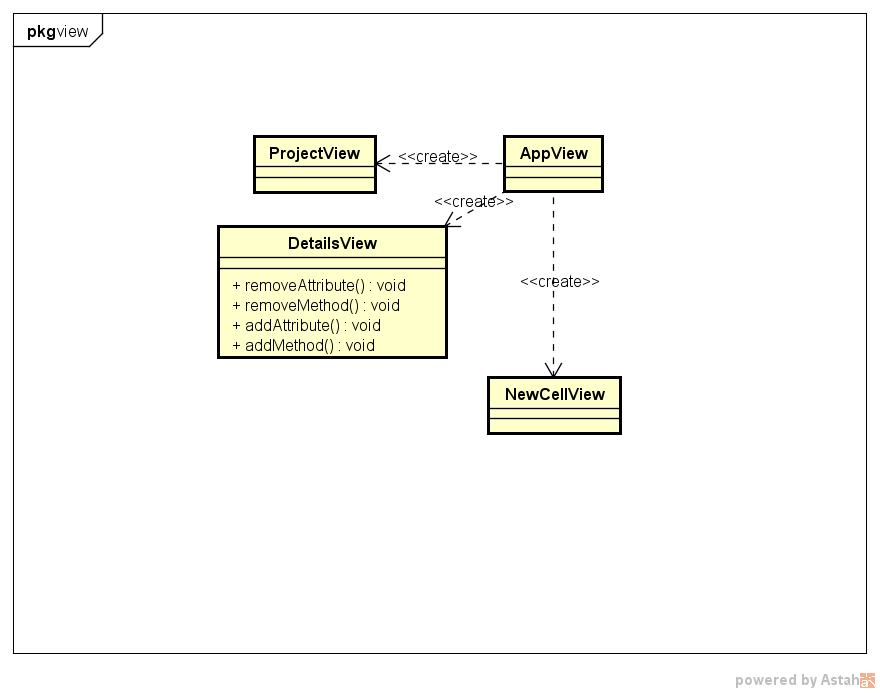
\includegraphics[width=1\textwidth]{img/client_view}}
	\caption{Diagramma package client::view}
\end{figure}
\begin{itemize}
\item \textbf{Descrizione}\\
Questo package raccoglie le classi che rappresentano i menù laterali e il \texttt{canvas} visualizzati dal browser, che popolano template e si sottoscrivono alla view tramite un pattern Observer. (I template non sono contenuti in questo package.)
\item \textbf{Padre}: \hyperref[\nogloxy{swedesigner::client}]{\nogloxy{\texttt{client}}}
\end{itemize}
\subsubsection{Classi}
\subsubsubsection{\nogloxy{swedesigner::client::view::AppView}}
\label{\nogloxy{swedesigner::client::view::AppView}}
\begin{itemize}
\item \textbf{Descrizione}\\
questa classe si occupa di gestire l'intera view dell'applicazione, componendo l'interfaccia principale e richiamando le altre view tramite il sistema a template di \backbonejs{}.
\item \textbf{Utilizzo}\\
essa è la prima classe costruita dall'entry point del programma.
\item \textbf{Relazioni con altre classi}:
\begin{itemize}
\item \textit{OUT} \hyperref[\nogloxy{swedesigner::client::model::ProjectCommand}]{\nogloxy{\texttt{ProjectCommand}}}\\
questa interfaccia descrive la struttura di un comando che viene chiamato da \texttt{AppView} quando l'utente decide di creare un nuovo progetto, di caricarne uno esistente, di salvarlo o di generare il codice dal diagramma. Il pattern realizzato è il pattern Command.
\item \textit{OUT} \hyperref[\nogloxy{swedesigner::client::model::ProjectModel}]{\nogloxy{\texttt{ProjectModel}}}\\
questa classe ci permette di aggiungere della logica alla collezione di tutti i diagrammi che possediamo.
\item \textit{OUT} \hyperref[\nogloxy{swedesigner::client::view::DetailsView}]{\nogloxy{\texttt{DetailsView}}}\\
questa classe si occupa di visualizzare tutti i campi di un blocco o di una relazione (come il nome di una classe, i suoi attributi, la condizione di un blocco \texttt{if} o il blocco di partenza di una relazione) permettendone anche la modifica. È possibile anche specificare uno stereotipo per la classe.

\item \textit{OUT} \hyperref[\nogloxy{swedesigner::client::view::NewCellView}]{\nogloxy{\texttt{NewCellView}}}\\
questa classe si occupa di visualizzare tutti i possibili blocchi e relazioni che si possono inserire nel diagramma delle classi o delle attività.
\item \textit{OUT} \hyperref[\nogloxy{swedesigner::client::view::ProjectView}]{\nogloxy{\texttt{ProjectView}}}\\
questa classe rappresenta l'area di disegno principale dell'applicazione, che necessita di essere cambiata tra diagramma delle classi e diagramma delle attività. 
\end{itemize}
\end{itemize}

\subsubsubsection{\nogloxy{swedesigner::client::view::DetailsView}}
\label{\nogloxy{swedesigner::client::view::DetailsView}}
\begin{itemize}
\item \textbf{Descrizione}\\
questa classe si occupa di visualizzare tutti i campi di un blocco o di una relazione (come il nome di una classe, i suoi attributi, la condizione di un blocco \texttt{if} o il blocco di partenza di una relazione) permettendone anche la modifica. È possibile anche specificare uno stereotipo per la classe.

\item \textbf{Utilizzo}\\
utilizza come model una tra le classi contenute nel package \texttt{celltypes}, in base alla selezione fatta dall'utente, e ne modifica i campi in base all'input. Essa eredita dalla \texttt{View} di \emph{Backbone.js} ed è una \emph{view} parallela alla \texttt{CellView} di ogni \texttt{Cell}, in quanto usa gli stessi modelli mostrando diversamente i dati.
In futuro, qualora l'implementazione di questa classe risulti troppo pesante o complicata da testare, è possibile subclassare questa classe in \emph{view} multiple e prevedere una nuova \emph{factory} di view.
\item \textbf{Relazioni con altre classi}:
\begin{itemize}
\item \textit{IN} \hyperref[\nogloxy{swedesigner::client::view::AppView}]{\nogloxy{\texttt{AppView}}}\\
questa classe si occupa di gestire l'intera view dell'applicazione, componendo l'interfaccia principale e richiamando le altre view tramite il sistema a template di \backbonejs{}.
\item \textit{OUT} \hyperref[\nogloxy{swedesigner::client::model::utility::ProjectStereotypes}]{\nogloxy{\texttt{ProjectStereotypes}}}\\
questa classe contiene al suo interno i possibili stereotipi utilizzabili recuperati dal server in modo asincrono. Conterrà una lista di elementi \textt{HxStereotype}.
\end{itemize}
\end{itemize}

\subsubsubsection{\nogloxy{swedesigner::client::view::NewCellView}}
\label{\nogloxy{swedesigner::client::view::NewCellView}}
\begin{itemize}
\item \textbf{Descrizione}\\
questa classe si occupa di visualizzare tutti i possibili blocchi e relazioni che si possono inserire nel diagramma delle classi o delle attività.
\item \textbf{Utilizzo}\\
utilizza \texttt{NewCellModel} per recuperare i blocchi e relazioni inseribili nel diagramma corrente (che può essere o delle classi o delle attività).
\item \textbf{Relazioni con altre classi}:
\begin{itemize}
\item \textit{IN} \hyperref[\nogloxy{swedesigner::client::view::AppView}]{\nogloxy{\texttt{AppView}}}\\
questa classe si occupa di gestire l'intera view dell'applicazione, componendo l'interfaccia principale e richiamando le altre view tramite il sistema a template di \backbonejs{}.
\item \textit{OUT} \hyperref[\nogloxy{swedesigner::client::model::NewCellModel}]{\nogloxy{\texttt{NewCellModel}}}\\
questa classe si occupa di fornire tutti i tipi di cell (tutti i blocchi e relazioni) da poter inserire nel diagramma corrente (o classi o attività).
\end{itemize}
\end{itemize}

\subsubsubsection{\nogloxy{swedesigner::client::view::ProjectView}}
\label{\nogloxy{swedesigner::client::view::ProjectView}}
\begin{itemize}
\item \textbf{Descrizione}\\
questa classe rappresenta l'area di disegno principale dell'applicazione, che necessita di essere cambiata tra diagramma delle classi e diagramma delle attività. 
\item \textbf{Utilizzo}\\
seleziona l'elemento \emph{Graph} da visualizzare. esso è presente nel relativo \emph{model}, che sarà di volta in volta cambiato selezionandolo dalla sua \emph{collection}.
\item \textbf{Relazioni con altre classi}:
\begin{itemize}
\item \textit{IN} \hyperref[\nogloxy{swedesigner::client::view::AppView}]{\nogloxy{\texttt{AppView}}}\\
questa classe si occupa di gestire l'intera view dell'applicazione, componendo l'interfaccia principale e richiamando le altre view tramite il sistema a template di \backbonejs{}.
\item \textit{OUT} \hyperref[\nogloxy{swedesigner::client::model::ProjectModel}]{\nogloxy{\texttt{ProjectModel}}}\\
questa classe ci permette di aggiungere della logica alla collezione di tutti i diagrammi che possediamo.
\end{itemize}
\end{itemize}

\begin{adjustwidth}{-3cm}{-3cm}
	\begin{figure}[H]
		\makebox[\textwidth][c]{
		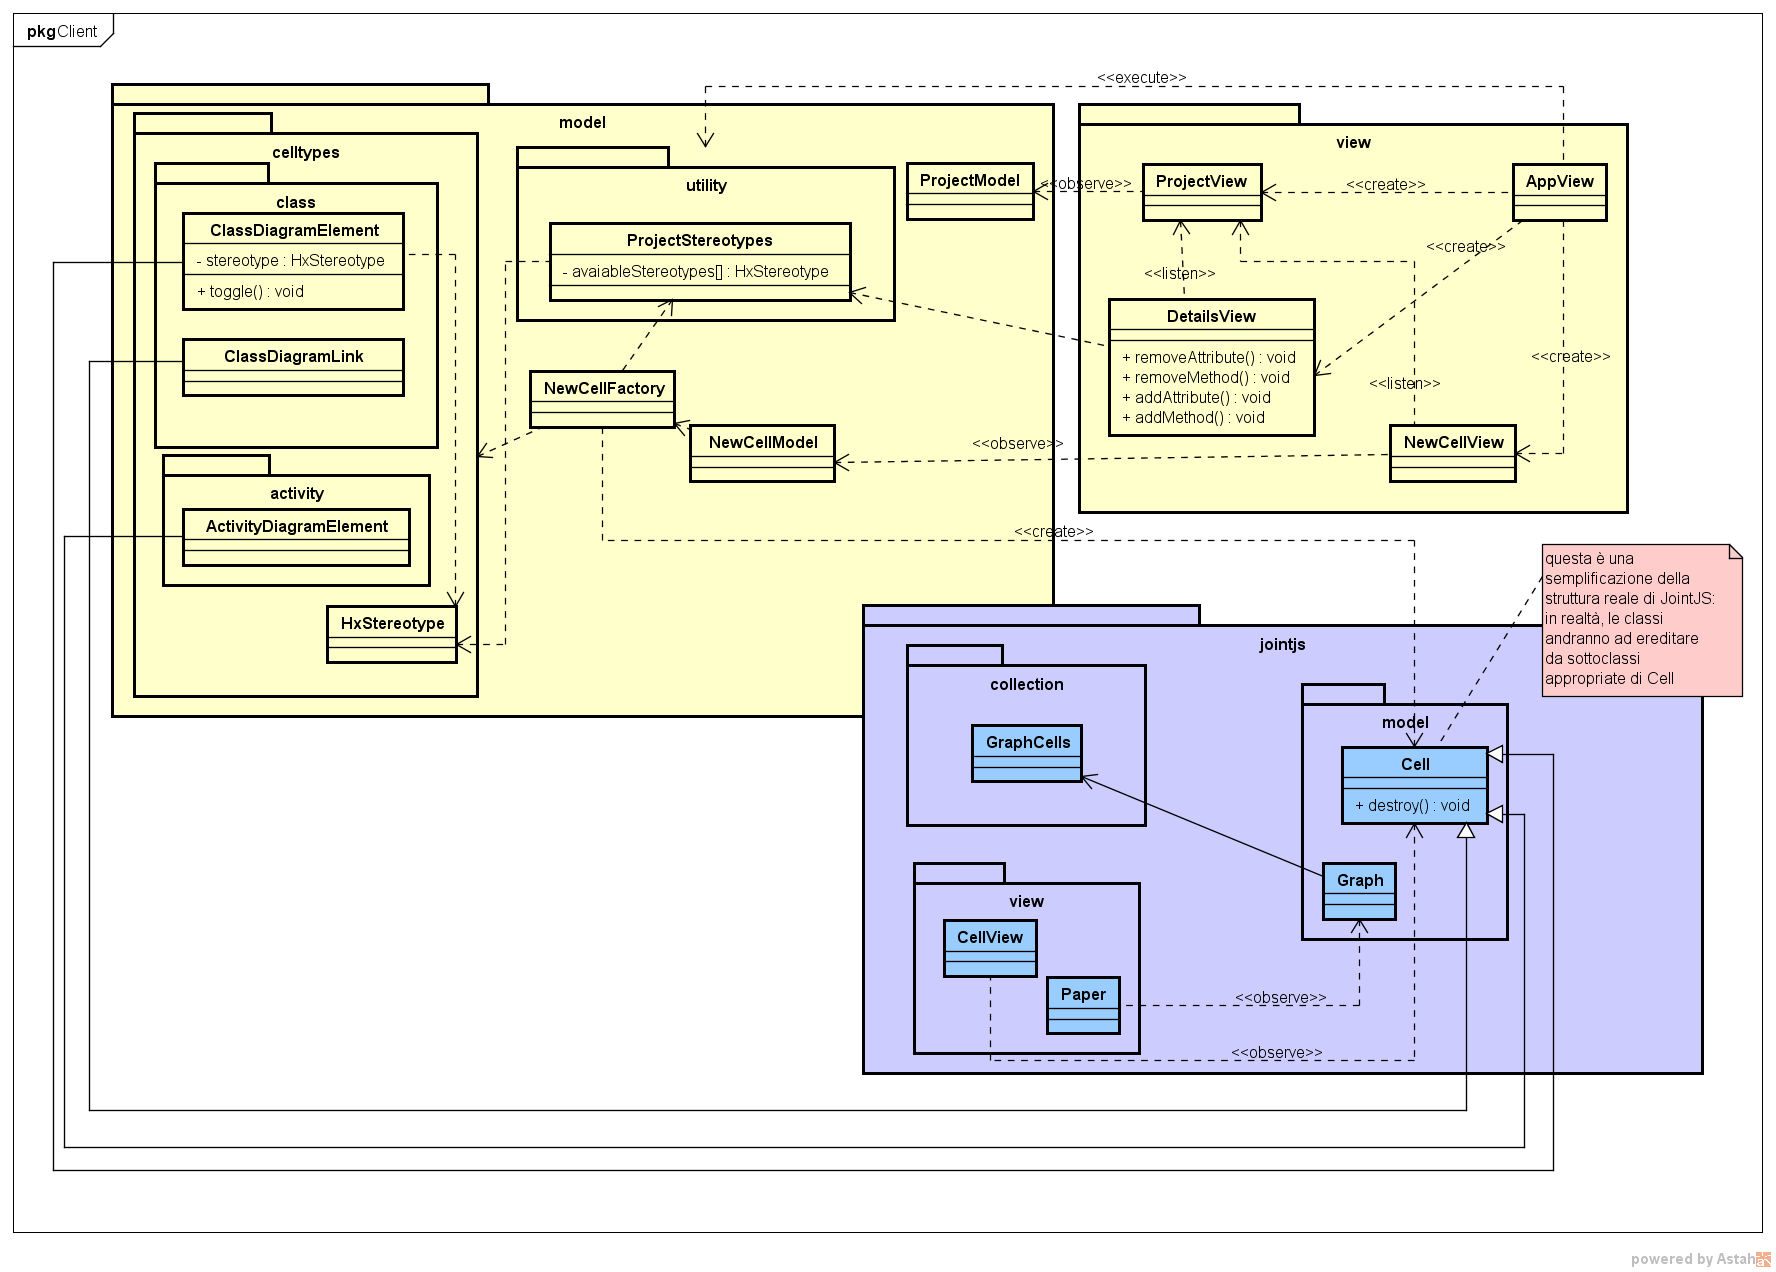
\includegraphics[width=1\textwidth]{img/client_hor}}
		\caption{Diagramma package client}
	\end{figure}
\end{adjustwidth}
